\chapter{Interpolation Polynomiale}
L'interpolation est une technique fondamentale en analyse numérique, qui s'illustre aussi bien dans la modélisation mathématique que dans la visualisation de données. Elle permet l'approximation d'un ensemble de données discrètes, à partir d'une fonction continue. L'objectif de ce TP est d'explorer deux méthodes d'interpolation, à savoir les méthodes de Newton et Neville. L'interpolation de Newton repose sur les différences divisées, tandis que la méthode de Neville utilise un schéma récursif pour construire un polynôme interpolateur. 
Dans ce rapport, nous explorerons en détail ces deux méthodes d'interpolation. Pour chacune d'entre-elles, nous commencerons par une présentation théorique, puis nous illustrerons nos propos avec un exemple pratique de résolution. Nous nous concentrerons ensuite sur leurs algorithmes respectifs, ainsi que sur leur implémentation en C. Nous analyserons enfin les résultats fournis par l'ordinateur des deux méthodes sur les 4 jeux d'essais présents en annexe de ce rapport, ainsi que les avantages et les limitations de chaque méthode.
\begin{figure}[h]
    \centering
    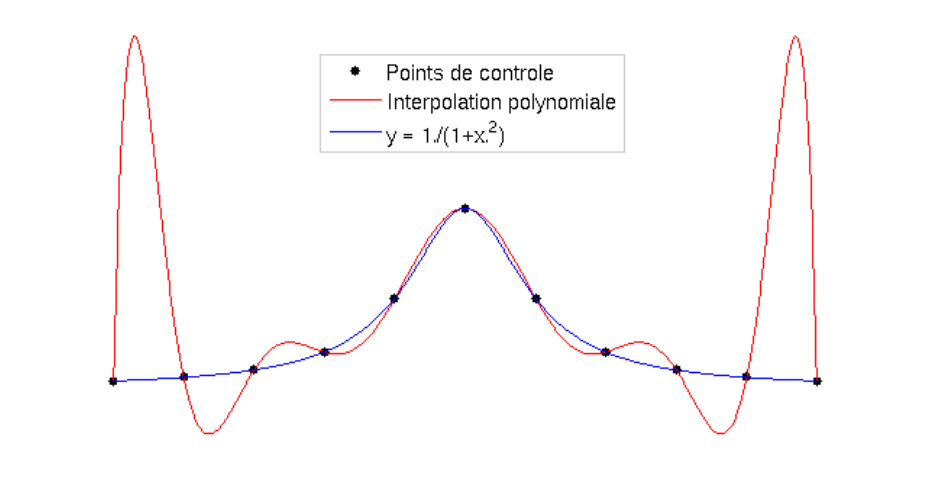
\includegraphics[width=1\textwidth]{chapter/interpolation.png}
    \caption{Exemple d'interpolation}
\end{figure}
\newpage
\section{Interpolation par la méthode de Neville}
\subsection{Présentation de la méthode}
La méthode de Neville est une technique d'interpolation qui permet d'approximer une fonction inconnue à partir de données discrètes. Elle repose sur un processus récursif de construction d'un polynôme interpolateur à partir des données initiales. À chaque étape, deux polynômes voisins sont combinés pour former un nouveau polynôme qui passe par certains points données. Cette méthode devient rapidement imprécise au fur et à mesure que le nombre de points augmente. Elle est en revanche efficace pour l'interpolation de petits ensembles de données.\vspace{6pt}\\
Considérons un ensemble de $n$ points donnés, notés $(x_i, y_i)$, où les $x_i$ sont deux à deux distincts. Nous cherchons à déterminer un polynôme d'interpolation $p(x)$ de degré $n-1$ au maximum, qui satisfait la condition suivante :
\begin{center}
    $p(x_i)=y_i$, \text{ avec   } $i=0, ..., n-1$
\end{center}
La méthode de Neville consiste à évaluer ce polynôme pour le point d'abscisse $x$.\\
Soit $p_k[x_i, ..., x_i+k](x)$ le polynôme de degré $k$ qui passe par les points $(x_i, y_i), ..., (x_{i+k}, y_{i+k})$. Alors $p_k[x_i, ..., x_{i+k}](x)$ vérifie la relation de récurrence suivante:\vspace{5pt}\\
\begin{equation*}
    \begin{cases}
        p_0[x_i](x)=y_i, \text{     avec  } 0\leqslant i< n \text{  et } k=0\vspace{6pt}\\
        p_k[x_i, ..., x_{i+k}](x)=\frac{(x-x_{i+k})p_{k-1}[x_i, ..., x_{i+k-1}](x)+(x_i-x)p_{k-1}[x_{i+1}, ..., x_{i+k}](x)}{x_i-x_{i+k}}, \text{     avec  } 1\leqslant k<n \text{ et } 0\leqslant i< n
    \end{cases}
\end{equation*}
Cette relation de récurrence permet de calculer $p_{n-1}[x_0, ..., x_{n-1}](x)$, qui est le polynôme recherché.
% Arbre à faire
\subsection{Résolution Manuelle}
\subsection{Algorithme}
\subsection{Implémentation en C}
\subsection{Exemples d'exécution}